\chapter{Casi d'uso}
In questa sezione sono elencati i casi d'uso del progetto MegAlexa dedotti da un'attenta indagine ed analisi da parte dei membri del gruppo sugli attori principali del sistema, sulle loro caratteristiche e possibilità.
Ogni caso d'uso è identificato da un codice univoco e possiede una struttura interna accuratamente definita nel documento Norme Di Progetto 
v1.0.0.
\section{Attori dei casi d'uso}
\textbf{Attori primari}
\begin{itemize}
	\item \textbf{Utente non autenticato}: si riferisce all'utente del sistema che non ha ancora eseguito il login;
	\item \textbf{Utente autenticato}: si riferisce all'utente del sistema che ha effettuato il login ed è stato autenticato.
\end{itemize}
\textbf{Attori secondari}
\begin{itemize}
	\item \textbf{Amazon}:/(da completare)
\end{itemize}
\section{Caso d'uso UC1: Scenario principale dell'utente non autenticato}
\begin{figure}[!ht]
	\centering
	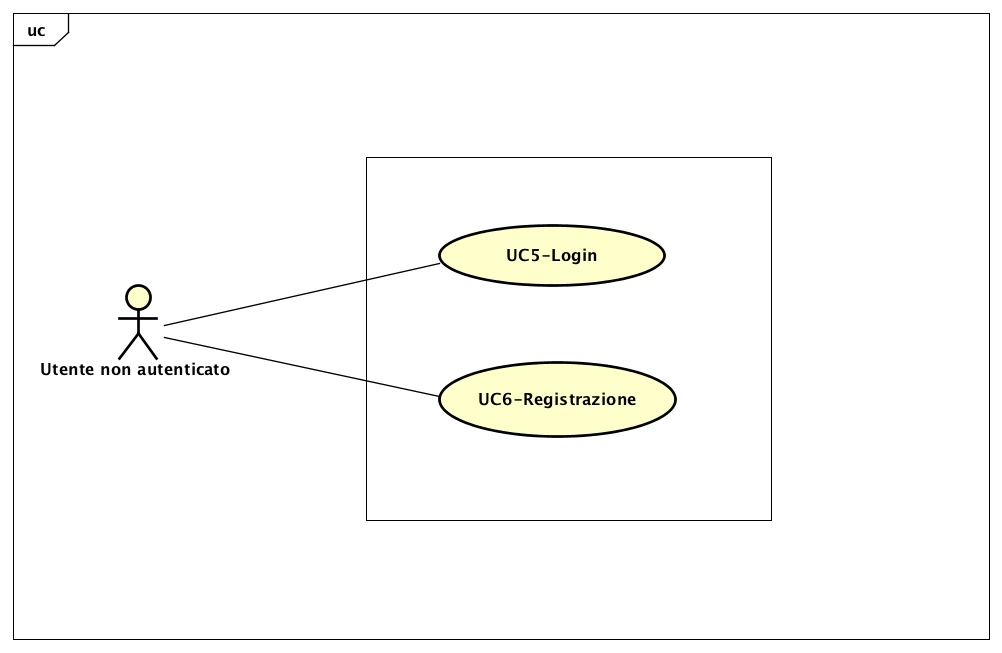
\includegraphics[scale=0.4]{Diagram/UC1.png}
	\caption{Scenario principale}\label{}
\end{figure}
\begin{itemize}
	\item \textbf{Attori primari}: Utente non autenticato;
	\item \textbf{Attori secondari}: DataBase??;
	\item \textbf{Descrizione:} Un utente non  autenticato può registrarsi al nostro servizio se non ha ancora un account o effettuare il login, nel caso fosse già registrato;
	\item \textbf{Precondizione:} L'applicazione è avviata e pronta all'uso;
	\item \textbf{Flusso principale degli eventi}:
	\begin{enumerate}
		\item L'utente ha la possibilità di: Registrazione (UC1.3);
		\item L'utente ha la possibilità di: Login (UC1.4).
	\end{enumerate}
	\item \textbf{Postcondizione}: L'applicazione ha ricevuto tutte le informazioni dell'utente non autenticato sulle operazioni che vuole eseguire.
\end{itemize}
\section{Caso d'uso UC1.1: Registrazione}
\begin{figure} [h]
	\centering
	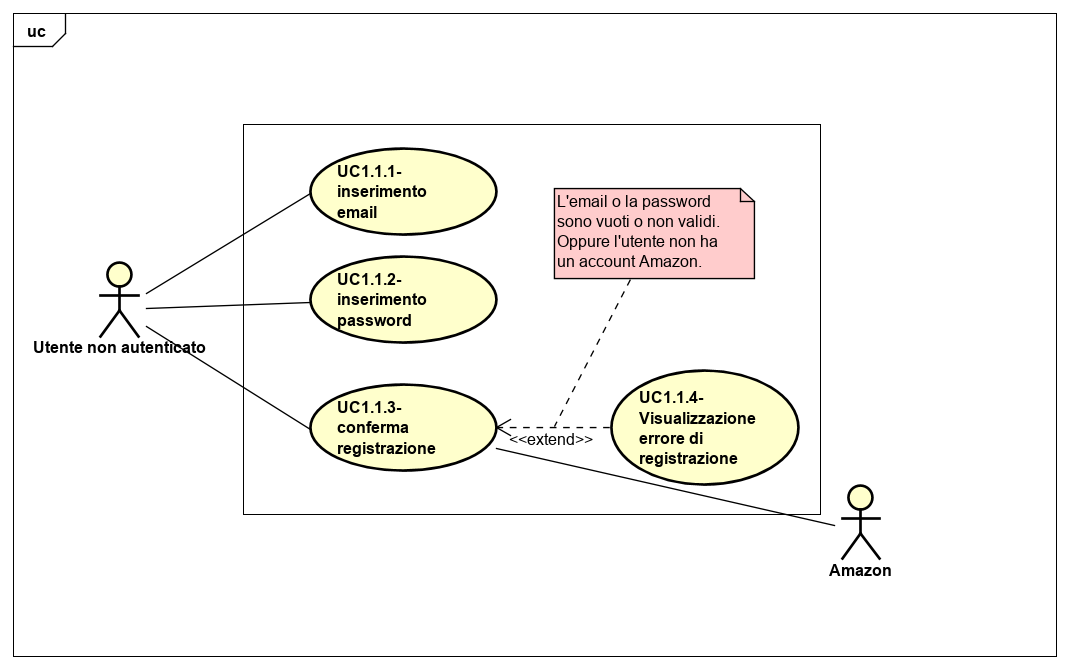
\includegraphics[scale=0.4]{./Diagram/UC1-1.png}
	\caption{Registrazione}\label{}
\end{figure}
\begin{itemize}
	\item \textbf{Attori primari}: Utente non autenticato;
	\item \textbf{Attori secondari}: Amazon;
	\item \textbf{Descrizione}: Per accedere al sistema è necessario possedere un account;
	\item \textbf{Precondizione}: L'attore non possiede un account per accedere al sistema;
	\item \textbf{Flusso principale degli eventi}: 
	\begin{enumerate}
		\item L'attore inserisce la propria email (UC1.1.1);
		\item L'attore inserisce la propria password (UC1.1.2);
		\item L'attore conferma la registrazione(UC1.1.3).
	\end{enumerate}
	\item \textbf{Scenario alternativo}: L'attore dopo aver confermato le proprie credenziali visualizza un messaggio d'errore (UC1.1.4);
	\item \textbf{Postcondizione}:E' stato creato un account per accedere al sistema.
		\item \textbf{Estensioni}:
	\begin{enumerate}
		\item	Visualizzazione errore di registrazione(UC1.1.4).
	\end{enumerate}
\end{itemize}

		\section{Caso d'uso UC1.1.1: Inserimento email}
\begin{itemize}
	\item \textbf{Attori primari}: Utente non autenticato;
	\item \textbf{Descrizione}: L'attore deve inserire la propria email per effettuare la  registrazione;
	\item \textbf{Precondizione}: Il sistema mostra il campo per l'inserimento della email;
	\item \textbf{Flusso principale degli eventi}: L'attore inserisce la propria email per effettuare la registrazione;
	\item \textbf{Postcondizione}: E' stata inserita l'email dell'attore nel campo opportuno.
\end{itemize}
\section{Caso d'uso UC1.1.2: Inserimento password}
\begin{itemize}
	\item \textbf{Attori primari}: Utente non autenticato;
	\item \textbf{Descrizione}: L'attore deve inserire la propria password per effettuare la registrazione;
	\item \textbf{Precondizione}: Il sistema mostra il campo per l'inserimento della password;
	\item \textbf{Flusso principale degli eventi}: L'attore inserisce la propria password per effettuare la registrazione;
	\item \textbf{Postcondizione}: È stata inserita la password dell'attore nel campo opportuno.
\end{itemize}

\section{Caso d'uso UC1.1.3: Conferma registrazione}
\begin{itemize}
	\item \textbf{Attori primari}: Utente non autenticato;
	\item \textbf{Descrizione}: L'attore dopo aver compilato i campi richiesti decide di confermare  la registrazione;
	\item \textbf{Precondizione}: Il sistema mostra un pulsante per confermare la registrazione;
	\item \textbf{Flusso principale degli eventi}:L'attore decide di confermare la registrazione per completarla.
	\item \textbf{Postcondizione:} Il sistema registra l'attore poiché questo ha confermato l'operazione.
	\item \textbf{Estensione:}
	\begin{itemize}
		\item Visualizzazione dell'errore di registrazione(UC1.1.4).
	\end{itemize}
\end{itemize}


\section{Caso d'uso UC1.1.4: Visualizzazione dell'errore di registrazione}
\begin{itemize}
	\item \textbf{Attori primari}: Utente non autenticato;
	\item \textbf{Descrizione}: L'attore visualizza un errore nel caso avesse compilato i campi con dati errati.
	\item \textbf{Precondizione}: Il sistema ha ricevuto campi dati errati: vuoti o non validi;
	\item \textbf{Flusso principale degli eventi}: L'attore visualizza il messaggio d'errore relativo al campo dato del:
	\begin{itemize}
		\item E-mail;
		\item Password;
	\end{itemize}
	\item \textbf{Postcondizione:} Il sistema mostra un messaggio d'errore per segnalare il tentativo di registrarsi con campi dati errati.
\end{itemize}

\section{Caso d'uso UC1.2: Login}
\begin{figure} [h]
	\centering
	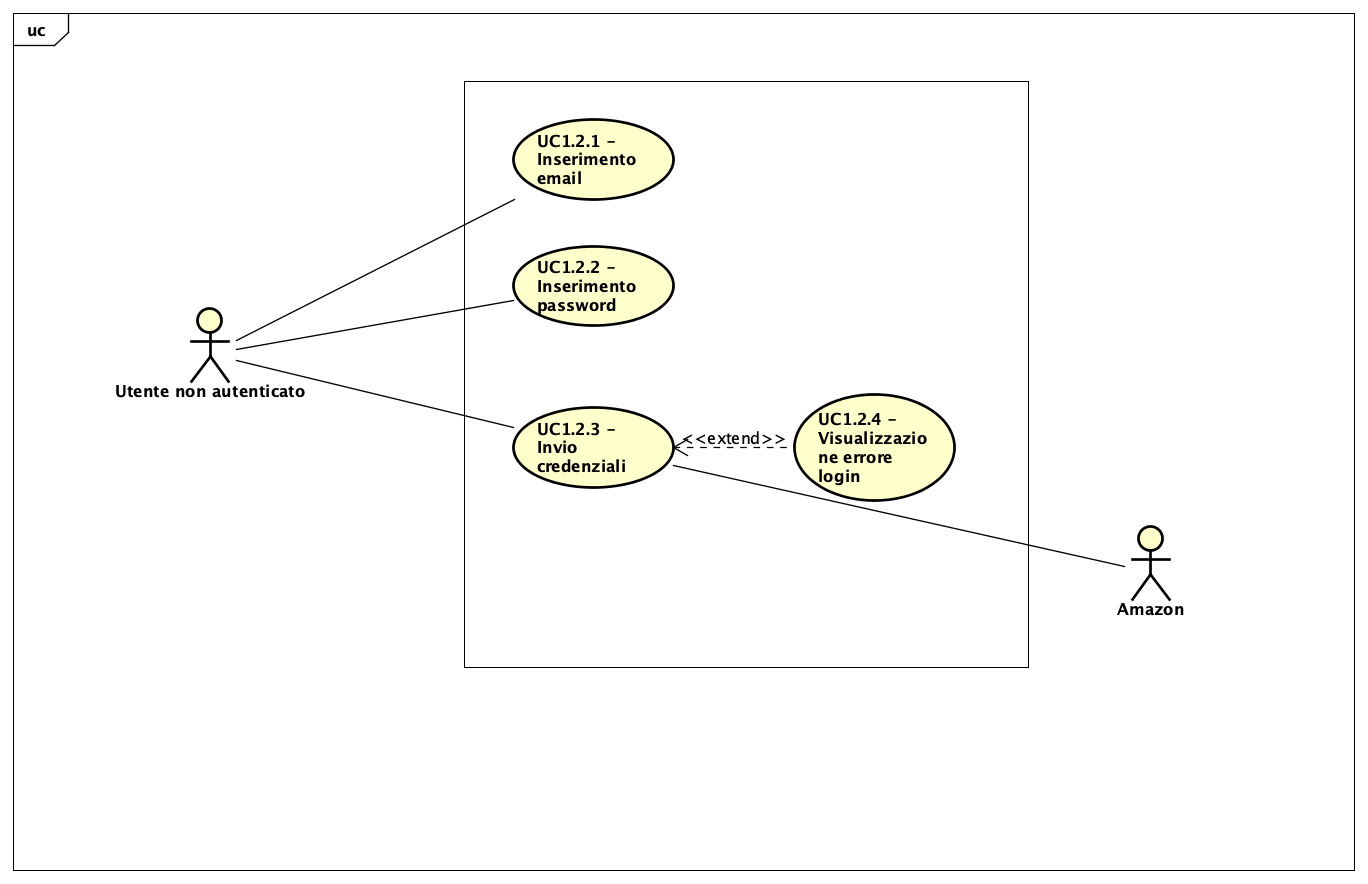
\includegraphics[scale=0.4]{./Diagram/UC1-2.png}
	\caption{Login}\label{}
\end{figure}
\begin{itemize}
	\item \textbf{Attori primari}: Utente non autenticato;
	\item \textbf{Attori secondari}: Amazon;
	\item \textbf{Descrizione}: Il sistema è avviato, ma è necessario effettuare il login per accedervi;
	\item \textbf{Precondizione}: Il sistema non permette l'accesso all'utente non autenticato;
	\item \textbf{Flusso principale degli eventi}:
	\begin{enumerate}
		\item L'utente inserisce la propria email (UC1.2.1);
		\item L'utente inserisce la propria password (UC1.2.2);
		\item L'utente invia le credenziali (UC1.2.3).
	\end{enumerate}
	\item \textbf{Scenario alternativo}: L'utente dopo aver inviato le proprie credenziali visualizza un messaggio d'errore (UC1.2.4);
	\item \textbf{Postcondizione}: Il sistema permette l'accesso all'utente che ora diventa un utente autenticato; 
	\item \textbf{Estensioni}:
	\begin{enumerate}
		\item	Visualizzazione errore login (UC1.2.4).
	\end{enumerate}
\end{itemize}

			
\section{Caso d'uso UC1.2.1: Inserimento email}
\begin{itemize}
	\item \textbf{Attori primari}: Utente non autenticato;
	\item \textbf{Descrizione}: L'utente inserisce la sua email per effettuare il login;
	\item \textbf{Precondizione}: Il sistema fa visualizzare il campo email;
	\item \textbf{Flusso principale degli eventi}: L'attore inserisce la sua mail per effettuare il login;
	\item \textbf{Postcondizione:} E' stata inserita la mail dell'attore nel campo predisposto. 
\end{itemize}

\section{Caso d'uso UC1.2.2: Inserimento password}
	\begin{itemize}
		\item \textbf{Attori primari}: Utente non autenticato;
		\item \textbf{Descrizione}: L'utente inserisce la sua password per effettuare il login;
		\item \textbf{Precondizione}: Il sistema fa visualizzare il campo password;
		\item \textbf{Flusso principale degli eventi}: L'attore inserisce la sua password per effettuare il login;
		\item \textbf{Postcondizione:} E' stata inserita la password dell'attore nel campo predisposto. 
	\end{itemize}
	\section{Caso d'uso UC1.2.3: Invio credenziali}
	\begin{itemize}
		\item \textbf{Attori primari}: Utente non autenticato;
		\item \textbf{Descrizione:} Dopo aver inserito tutti i dati l'utente conferma il login;
		\item \textbf{Precondizione}: Il sistema far visualizzare la pagina di login;
		\item \textbf{Flusso principale degli eventi}: L'attore dopo aver inserito le credenziali può confermare il login;
		\item \textbf{Postcondizione}: L'utente è riconosciuto dal sistema come utente autenticato;
		\item \textbf{Scenari alternativi}: L'utente inserisce credenziali errate e viene visualizzato un messaggio d'errore;
		\item \textbf{Estensioni}:
		\begin{enumerate}
			\item Visualizzazione errore login (UC1.2.4).
		\end{enumerate} 
	\end{itemize}
	\section{Caso d'uso UC1.2.4: Visualizzazione errore login}
		\begin{itemize}
			\item \textbf{Attori primari}: Utente non autenticato;
			\item \textbf{Descrizione:} L'attore può aver inserito delle credenziali errate;
			\item \textbf{Precondizione}: Il sistema ha ricevuto campi dati errati;
			\item \textbf{Flusso principale degli eventi}: L'attore visualizza un messaggio d'errore;
			\item \textbf{Postcondizione:} L'utente non è riconosciuto dal sistema.
		\end{itemize}
		\section{Caso d'uso UC1.1.2: Inserimento cognome}
		\begin{itemize}
			\item \textbf{Attori primari}: Utente non autenticato;
			\item \textbf{Descrizione:} L'attore deve inserire il proprio cognome per effettuare la registrazione;
			\item \textbf{Precondizione}: Il sistema mostra il campo per l'inserimento del cognome;
			\item \textbf{Flusso principale degli eventi}: L'attore inserisce il proprio cognome per effettuare la registrazione;
			\item \textbf{Postcondizione}: E' stato inserito il nome dell'attore nel campo opportuno.
		\end{itemize}
		\section{Caso d'uso UC1.1.3: Inserimento e-mail}
		\begin{itemize}
			\item \textbf{Attori primari}: Utente non autenticato;
			\item \textbf{Descrizione}: L'attore deve inserire la propria e-mail per effettuare la  registrazione;
			\item \textbf{Precondizione}: Il sistema mostra il campo per l'inserimento della e-mail;
			\item \textbf{Flusso principale degli eventi}: L'attore inserisce la propria e-mail per effettuare la registrazione;
			\item \textbf{Postcondizione}: E' stata inserita l'e-mail dell'attore nel campo opportuno.
		\end{itemize}
		\section{Caso d'uso UC1.1.4: Inserimento password}
		\begin{itemize}
			\item \textbf{Attori primari}: Utente non autenticato;
			\item \textbf{Descrizione} :L'attore deve inserire la propria password per effettuare la registrazione;
			\item \textbf{Precondizione}:Il sistema mostra il campo per l'inserimento della password;
			\item \textbf{Flusso principale degli eventi}:L'attore inserisce la propria password per effettuare la registrazione;
			\item \textbf{Postcondizione}: E' stata inserita la password dell'attore nel campo opportuno.
		\end{itemize}
		\section{Caso d'uso UC1.1.5: Inserimento conferma password}
		\begin{itemize}
			\item \textbf{Attori primari}: Utente non autenticato;
			\item \textbf{Descrizione:} L'attore deve inserire la conferma della password per effettuare la registrazione;
			\item \textbf{Precondizione}:Il sistema mostra il campo per l'inserimento della conferma della password;
			\item \textbf{Flusso principale degli eventi}:L'attore inserisce la conferma della password per effettuare la registrazione;
			\item \textbf{Postcondizione}: E' stata inserita la conferma della password dell'attore nel campo opportuno.
		\end{itemize}
		\section{Caso d'uso UC1.1.6: Annullamento registrazione}
		\begin{itemize}
			\item \textbf{Attori primari}: Utente non autenticato;
			\item \textbf{Descrizione:} L'attore decide di annullare la registrazione in corso;
			\item \textbf{Precondizione}:Il sistema mostra un pulsante per annullare la  registrazione;
			\item \textbf{Flusso principale degli eventi}:L'attore decide di annullare la registrazione che stava eseguendo;
			\item \textbf{Postcondizione}: Il sistema non registra l'attore poichè questo ha annullato l'operazione.
		\end{itemize}
		\section{Caso d'uso UC1.1.7: Conferma registrazione}
		\begin{itemize}
			\item \textbf{Attori primari}: Utente non autenticato;
			\item \textbf{Descrizione}: L'attore dopo aver compilato i campi richiesti decide di confermare  la registrazione;
			\item \textbf{Precondizione}: Il sistema mostra un pulsante per confermare la registrazione;
			\item \textbf{Flusso principale degli eventi}:L'attore decide di confermare la registrazione per completarla.
			\item \textbf{Postcondizione:} Il sistema registra l'attore poichè questo ha confermato l'operazione.
			\item \textbf{Estensione:}
			\begin{itemize}
				\item Visualizzazione dell'errore di registrazione(UC)
			\end{itemize}
		\end{itemize}
		\section{Caso d'uso UC1.1.8: Visualizzazione dell'errore di registrazione}
		\begin{itemize}
			\item \textbf{Attori primari}: Utente non autenticato;
			\item \textbf{Descrizione}: L'attore visualizza un errore nel caso avesse compilato i campi con dati errati.
			\item \textbf{Precondizione}: Il sistema ha ricevuto campi dati errati: vuoti o non validi;
			\item \textbf{Flusso principale degli eventi}: L'attore visualizza il messaggio d'errore relativo al campo dato  del:
			\begin{itemize}
				\item Nome;
				\item Cognome;
				\item E-mail;
				\item Password;
				\item Conferma Password;
			\end{itemize}
			\item \textbf{Postcondizione:} Il sistema mostra un messaggio d'errore per segnalare il tentativo di registrarsi con campi dati errati.
		\end{itemize}
		\section{Caso d'uso UC1.2: Login}
		\begin{itemize}
			\item \textbf{Attori primari}: Utente non autenticato;
			\item \textbf{Attori secondari}: ;
			\item \textbf{Descrizione:} L'utente richiede il login al sistema;
			\item \textbf{Precondizione:} Il sistema non permette l'accesso all'utente non autenticato;
			\item \textbf{Flusso principale degli eventi:} L'utente effettua il login.
			\item \textbf{Postcondizione:} Il sistema consente l'accesso all'utente che ora è autenticato.
		\end{itemize}
		\section{Caso d'uso UC2: Scenario principale dell'utente autenticato}
		\begin{figure} [h]
			\centering
			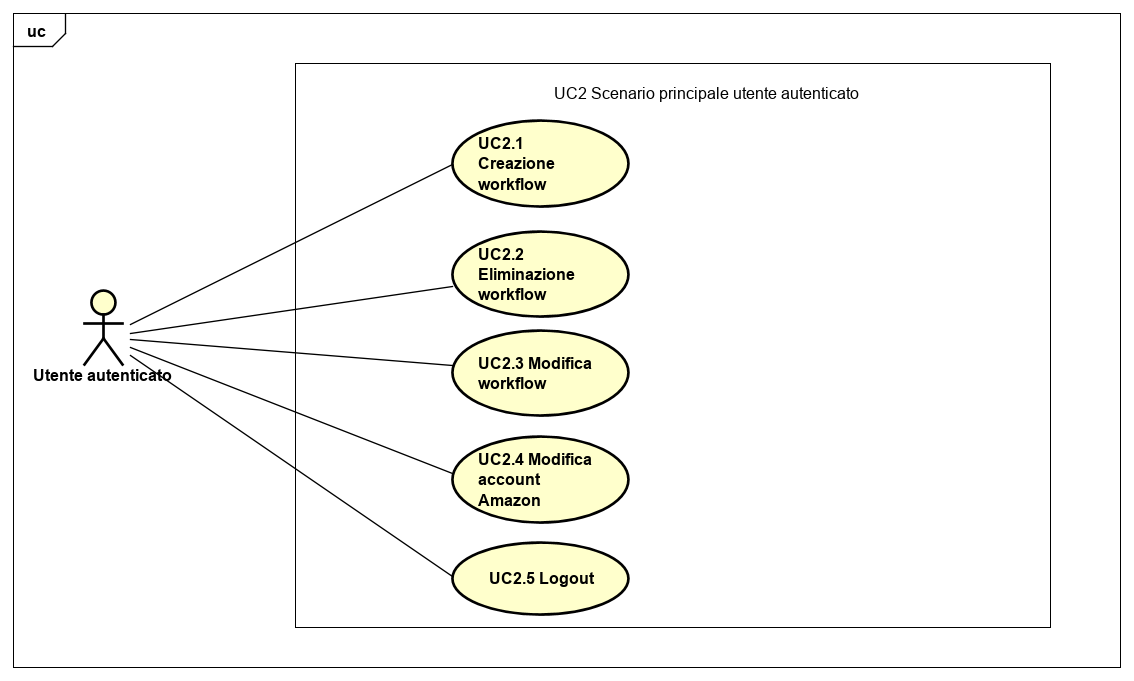
\includegraphics[scale=0.4]{./Diagram/UC2.png}
			\caption{Scenario principale dell'utente autenticato }\label{}
		\end{figure}
		\begin{itemize}
			\item \textbf{Attori primari}: Utente autenticato;
			\item \textbf{Descrizione:} L'attore può creare, modificare ed eliminare un workflow, modificare i propri dati personali ed eseguire il logout.
			\item \textbf{Precondizione:} Il sistema mostra la pagina principale per l'utente autenticato.
			\item \textbf{Flusso principale degli eventi:}
			\begin{enumerate}
				\item l'utente può creare un Workflow (UC2.1);
				\item l'utente può eliminare un Workflow (UC2.2);
				\item l'utente può modificare un Workflow (UC2.3);
				\item l'utente può modificare l'account Amazon (UC2.4);
				\item l'utente può effettuare il Logout (UC2.5).
			\end{enumerate}
			\item \textbf{Postcondizione:} Il sistema ha ricevuto le informazioni riguardanti i comandi che l'utente vuole eseguire.
		\end{itemize}
		\section{Caso d'uso UC2.1: Creazione workflow}
		\begin{figure} [h]
			\centering
			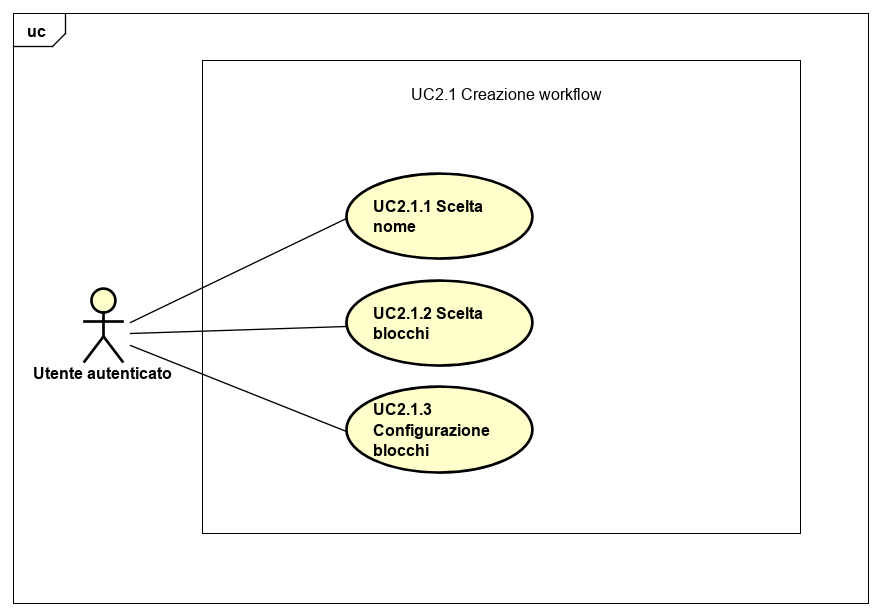
\includegraphics[scale=0.4]{./Diagram/UC2-1.png}
			\caption{Scenario principale dell'utente autenticato }\label{}
		\end{figure}
		\begin{itemize}
			\item \textbf{Attori primari}: Utente autenticato;
			\item \textbf{Descrizione:} L'attore può creare un workflow selezionando e configurando i blocchi disponibili;
			\item \textbf{Precondizione:} Il sistema mette a dispozione un form per la creazione di un workflow;
			\item \textbf{Flusso principale degli eventi:}
			\begin{enumerate}
				\item l'utente sceglie il nome del workflow (UC2.1.1);
				\item l'utente seleziona quali blocchi vuole usare (UC2.1.2);
				\item l'utente configura i blocchi selezionani (UC2.1.3);
			\end{enumerate}
			\item \textbf{Postcondizione:} Il sistema contiene il workflow desiderato dall'attore.
		\end{itemize}
		\section{Caso d'uso UC2.1.1: Scelta nome }
		\begin{itemize}
			\item \textbf{Attori primari}: Utente autenticato;
			\item \textbf{Descrizione:} L'attore inserisce il nome del workflow;
			\item \textbf{Precondizione:} Il sistema mette a dispozione un campo per l'inserimento del nome;
			\item \textbf{Flusso principale degli eventi:}
			\begin{enumerate}
				\item l'utente inserisce il nome del workflow;
			\end{enumerate}
			\item \textbf{Postcondizione:} Il form di creazione del workflow contiene il nome del workflow.
		\end{itemize}
		\section{Caso d'uso UC2.1.2: Scelta blocchi }
		\begin{itemize}
			\item \textbf{Attori primari}: Utente autenticato.
			\item \textbf{Descrizione:} L'attore sceglie i blocchi che compongono il workflow.
			\item \textbf{Precondizione:} Il sistema mette a disposizione un form per l'inserimento dei blocchi e una lista di blocchi disponibili.
			\item \textbf{Flusso principale degli eventi:}
			\begin{enumerate}
				\item l'attore inserisce i blocchi nel form e li ordina come preferisce;
			\end{enumerate}
			\item \textbf{Postcondizione:} Il workflow contiene i blocchi desiderati dall'utente.
		\end{itemize}
		\section{Caso d'uso UC2.1.3: Configurazione blocchi }
		\begin{itemize}
			\item \textbf{Attori primari}: Utente autenticato.
			\item \textbf{Descrizione:} L'attore configura i blocchi che compongono il workflow.
			\item \textbf{Precondizione:} Il sistema mette a disposizione un form per la configurazione dei blocchi.
			\item \textbf{Flusso principale degli eventi:}
			\begin{enumerate}
				\item l'attore configura i blocchi;
			\end{enumerate}
			\item \textbf{Postcondizione:} Il workflow contiene solo blocchi confugrati.
		\end{itemize}
		\section{Caso d'uso UC2.2: Eliminazione workflow}
		\begin{itemize}
			\item \textbf{Attori primari}: Utente autenticato.
			\item \textbf{Descrizione:} L'attore elimina un workflow.
			\item \textbf{Precondizione:} Il sistema mette a dispozione un comando per eliminare un workflow.
			\item \textbf{Flusso principale degli eventi:}
			\begin{enumerate}
				\item l'utente seleziona il comando per eliminare workflow che vuole rimuovere;
			\end{enumerate}
			\item \textbf{Postcondizione:} Il workflow che l'attore voleva eliminare è stato rimosso dal sistema.
		\end{itemize}
		\section{Caso d'uso UC2.3: Modifica workflow}
		\begin{figure} [h]
			\centering
			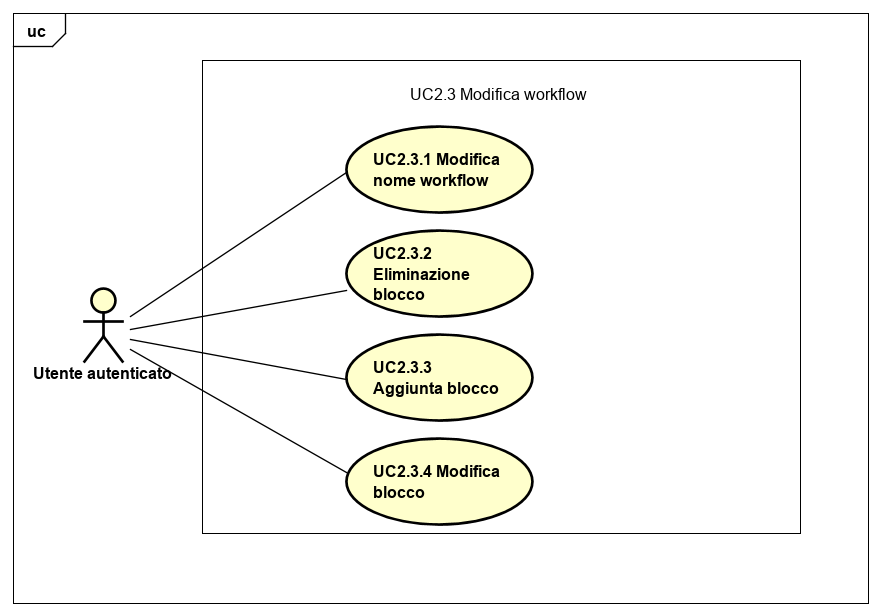
\includegraphics[scale=0.4]{./Diagram/UC2-3.png}
			\caption{Modifica workflow }\label{}
		\end{figure}
		\begin{itemize}
			\item \textbf{Attori primari}: Utente autenticato.
			\item \textbf{Descrizione:} L'attore modifica un workflow.
			\item \textbf{Precondizione:} Il sistema mette a dispozione un form per la modifica di un workflow.
			\item \textbf{Flusso principale degli eventi:}
			\begin{enumerate}
				\item l'attore può cambiare il nome del workflow (UC2.3.1);
				\item l'attore può eliminare un blocco dal workflow (UC2.3.2);
				\item l'attore può aggiungere un blocco nel workflow (UC2.3.3);
				\item l'attore può modificare la configurazione di un blocco presente nel workflow (UC2.3.4);
				\item 
			\end{enumerate}
			\item \textbf{Postcondizione:} Il workflow è stato modificato.
		\end{itemize}
		\section{Caso d'uso UC2.3.1: Modifica nome workflow}
		\begin{itemize}
			\item \textbf{Attori primari}: Utente autenticato.
			\item \textbf{Descrizione:} L'attore modifica il nome del workflow.
			\item \textbf{Precondizione:} Il sistema mette a dispozione un campo per l'inserimento del nuovo nome.
			\item \textbf{Flusso principale degli eventi:}
			\begin{enumerate}
				\item l'attore inserisce il nuovo nome del workflow;
			\end{enumerate}
			\item \textbf{Postcondizione:} Il form di creazione del workflow contiene il nuovo nome del workflow.
		\end{itemize}
		\section{Caso d'uso UC2.3.2: Eliminazione blocco }
		\begin{itemize}
			\item \textbf{Attori primari}: Utente autenticato.
			\item \textbf{Descrizione:} L'attore rimuove il blocco che non desidera più dal workflow.
			\item \textbf{Precondizione:} Il sistema fornisce un comando per l'eliminazione del blocco.
			\item \textbf{Flusso principale degli eventi:}
			\begin{enumerate}
				\item l'attore elimina il blocco;
			\end{enumerate}
			\item \textbf{Postcondizione:} Il workflow non contiene più il blocco indesiderato dall'attore.
		\end{itemize}
		\section{Caso d'uso UC2.3.3: Aggiunta blocco }
		\begin{itemize}
			\item \textbf{Attori primari}: Utente autenticato.
			\item \textbf{Descrizione:} L'attore aggiunge il nuovo blocco al workflow.
			\item \textbf{Precondizione:} Il sistema mette a disposizione un form per l'aggiunta del blocco.
			\item \textbf{Flusso principale degli eventi:}
			\begin{enumerate}
				\item l'attore aggiunge il blocco;
				\item l'attore configura il nuovo blocco;
			\end{enumerate}
			\item \textbf{Postcondizione:} Il workflow contiene il nuovo blocco configurato.
		\end{itemize}
		\section{Caso d'uso UC2.3.4: Modifica blocco }
		\begin{itemize}
			\item \textbf{Attori primari}: Utente autenticato.
			\item \textbf{Descrizione:} L'attore modifica la configurazione del blocco che compone il workflow.
			\item \textbf{Precondizione:} Il sistema mette a disposizione un form per la modifca dei blocchi.
			\item \textbf{Flusso principale degli eventi:}
			\begin{enumerate}
				\item l'attore modifica la configurazione del blocco;
			\end{enumerate}
			\item \textbf{Postcondizione:} Il blocco desiderato dall'attore è stato riconfigurato.
		\end{itemize}
		\section{Caso d'uso UC2.4: Modifica account Amazon }
		\begin{itemize}
			\item \textbf{Attori primari}: Utente autenticato.
			\item \textbf{Descrizione:} L'attore cambia il proprio account Amazon.
			\item \textbf{Precondizione:} Il sistema mette a disposizione un form per la modifica dell'account Amazon.
			\item \textbf{Flusso principale degli eventi:}
			\begin{enumerate}
				\item l'attore, attraverso il form di Amazon, sceglie il nuovo account;
			\end{enumerate}
			\item \textbf{Postcondizione:} Il sistema è collegato al nuovo account Amazon.
			\item \textbf{Estensione:}
			\begin{itemize}
				\item Visualizzazione dell'errore di cambio Account(UC2.4.1);
			\end{itemize}
		\end{itemize}
		\section{Caso d'uso UC2.4.1: Errore di cambio account Amazon }
		\begin{itemize}
			\item \textbf{Attori primari}: Utente autenticato.
			\item \textbf{Descrizione:} L'attore ha inserito dei dati non corretti e non riesce a collegarsi al nuovo account Amazon.
			\item \textbf{Precondizione:} Il sistema non riesce a collegarsi all'account Amazon.
			\item \textbf{Flusso principale degli eventi:}
			\begin{enumerate}
				\item l'attore può inserire nuovamente i dati nel form di Amazon;
				\item l'attore può tornare al vecchio account Amazon;
			\end{enumerate}
			\item \textbf{Postcondizione:} Il sistema è correttamente collegato a un account Amazon.
		\end{itemize}
		\section{Caso d'uso UC2.5: Logout }
		\begin{itemize}
			\item \textbf{Attori primari}: Utente autenticato.
			\item \textbf{Descrizione:} L'attore effettua il logout dall'applicazione.
			\item \textbf{Precondizione:} Il sistema fornisce un metodo per permettere all'utente di disconnettersi dal sistema.
			\item \textbf{Flusso principale degli eventi:}
			\begin{enumerate}
				\item l'attore si disconnette dal sistema;
			\end{enumerate}
			\item \textbf{Postcondizione:} Il sistema non riconosce più l'utente.
		\end{itemize}
			

			






